%
% File NLP4MusA.tex
%
%% Based on the style files for NLP4MusA 2020, which were
%% Based on the style files for ACL 2018, NAACL 2018/19, which were
%% Based on the style files for ACL-2015, with some improvements
%%  taken from the NAACL-2016 style
%% Based on the style files for ACL-2014, which were, in turn,
%% based on ACL-2013, ACL-2012, ACL-2011, ACL-2010, ACL-IJCNLP-2009,
%% EACL-2009, IJCNLP-2008...
%% Based on the style files for EACL 2006 by 
%%e.agirre@ehu.es or Sergi.Balari@uab.es
%% and that of ACL 08 by Joakim Nivre and Noah Smith

\documentclass[11pt,a4paper]{article}
\usepackage[hyperref]{nlp4MusA}
\usepackage{times}
\usepackage{latexsym}
\usepackage{graphicx}
\usepackage{mathtools}  % amsmath with extensions
\usepackage{amsfonts}  % (otherwise \mathbb does nothing)
\usepackage{url}


%\aclfinalcopy % Uncomment this line for the final submission
%\def\aclpaperid{100} %  Enter the acl Paper ID here

%\setlength\titlebox{5cm}
% You can expand the titlebox if you need extra space
% to show all the authors. Please do not make the titlebox
% smaller than 5cm (the original size); we will check this
% in the camera-ready version and ask you to change it back.

\newcommand\BibTeX{B\textsc{ib}\TeX}


\title{Shift-Invariant Dictionary Learning using Temporal CONV-WTA Autoencoders for Discovering Music Relations }

\author{First Author \\
  Affiliation / Address line 1 \\
  Affiliation / Address line 2 \\
  Affiliation / Address line 3 \\
  \texttt{email@domain} \\\And
  Second Author \\
  Affiliation / Address line 1 \\
  Affiliation / Address line 2 \\
  Affiliation / Address line 3 \\
  \texttt{email@domain} \\}

\date{}

\begin{document}
\maketitle
\begin{abstract}
The temporal structure  of music is full of shift-invariant patterns (e.g. motifs, ostinatos, loops, etc.). We propose using a Temporal Convolutional Winner-Take-All (CONV-WTA) autoencoder to find a shift-invariant dictionary to represent symbolic, multivariate, musical signals. The model learns to represent fixed length drum beats and variable length piano music. We discuss applications of this sparse representation such as de-noising musical ideas, unsupervised learning of composer styles, and music generation. To assist in related work we include interactive code along with the trained models

\end{abstract}

\section{Introduction}

The dictionary learning framework aims at finding a sparse representation of the input data (sparse coding) in the form of a linear combination of basic elements called atoms. In doing so, sparse coding enables faster inference and easier interpretability thanks to its lightweight stored memory, encoding of prior knowledge in the sparsity patterns, and discerning patterns in an informed and principled manner.  

 Sparse dictionary learning has led to state-of-art results in various tasks including image and video processing, texture synthesis \cite{Peyre2009}, and unsupervised clustering \cite{Ramrez2010ClassificationAC}. In evaluations with the Bag-of-Words model \cite{7439823}, sparse coding was found empirically to outperform other coding approaches on category recognition tasks.  

When applied to music, the ability to distil complex data structures down to sets of dictionaries—salient features of a specific performer or music, has a multitude of applications. Music transcription and classification tasks have seen a strong usage of sparse dictionary learning in the past \cite{Grosse2007} \cite{Costantini2013}, \cite{Blumensath2006}, \cite{SrinivasM2014}, \cite{Srinivas2014}, \cite{Cogliati2016}. Nonetheless, we have yet to see a study that harnesses the advantages of sparse representation for the purpose of music creation. Instead, the popular methods for discovering music relations and achieving music generation have been a transformer with some sort of attention mechanism or other recurrent architectures. For instance, \cite{JiangJunyan2020} uses an attention module that is tailored to the discovery of sequence level relations in music, while studies like \cite{Roberts2018} uses the recurrent variational autoencoder and a hierarchical decoder in order to model long-term musical structures. In our study, we explore applications of sparse representation such as de-noising musical ideas, unsupervised learning of composer styles, and music generation.

 

% ConvNets were subsequently
%applied to NLP tasks such as part-of-speech tagging and
%semantic role labelling (Collobert ; Weston, 2008; Collobert et al., 2011; dos Santos ; Zadrozny, 2014). More
%recently, convolutional networks were applied to sentence
%classification (Kalchbrenner et al., 2014; Kim, 2014) and
%document classification (Zhang et al., 2015; Conneau et al.,
%2017; Johnson ; Zhang, 2015; 2017). Particularly inspiring
%for our work are the recent applications of convolutional
%architectures to machine translation (Kalchbrenner et al.,
%2016; Gehring et al., 2017a;b), audio synthesis (van den
%Oord et al., 2016), and language modeling (Dauphin et al.,
%2017).


\section{Preliminaries}


\subsection{ Dictionary learning  }
Given the data: $ X=\left[x_{1}, \ldots, x_{K}\right], x_{i} \in \mathbb{R}^{d} $. 
We want a dictionary $\mathbf{D} \in \mathbb{R}^{d \times n}: D=\left[d_{1}, \ldots, d_{n}\right]$ ,
and a representation $R=\left[r_{1}, \ldots, r_{K}\right], r_{i} \in \mathbb{R}^{n}$ such that the reconstruction $\|X-\mathbf{D} R\|_{F}^{2}$ is minimized and $r_{i}$ are sparsed. The optimization problem can be formulated as: 

$\underset{\mathbf{D} \in \mathcal{C}, r_{i} \in \mathbb{R}^{n}, \lambda>0} {\operatorname{argmin}} \sum_{i=1}^{K}\left\|x_{i}-\mathbf{D} r_{i}\right\|_{2}^{2}+\lambda\left\|r_{i}\right\|_{0}$ \\   $\mathcal{C} \equiv\left\{\mathbf{D} \in \mathbb{R}^{d \times n}:\left\|d_{i}\right\|_{2} \leq 1 \forall i=1, \ldots, n\right\} $
\\ \\
There are various methods to solve this problem, however this formulation does not look for shift- invariant features. The dictionary components are the same size as the original signal we are seeking to reconstruct.

\subsection{ Shift-invariant Dictionary Learning (SIDL)  }

Shift-invariant dictionary learning (SIDL) refers to the problem of discovering a latent basis that captures local patterns at different locations of input signal, and a sparse coding for each sequence as a linear combination of these elements \cite{Zheng2016} In previous works, various shift-invariant dictionary learning (SIDL) methods have been employed to discover local patterns that are embedded across a longer time series in sequential data such as audio signals  \cite{Grosse2007}  

This has a similar formulation as DL except that in order to reconstruct the signal, we need to stride along the input signal:  \\
$\mathbf{D} r_{i} \longrightarrow \sum_{k=1}^{K} (\boldsymbol{r}_{i})_{k} T\left(\mathbf{d}_{k}, t_{i k}\right)$
\\
where \\
$T(\mathbf{d}, t) \ =\begin{cases}\mathbf{d}_{i-t} & \text { if } 1 \leq i-t \leq q \\ 0 & \text { otherwise }\end{cases}$

here $t_{i k}$ corresponds to the first location where $d_k$ matches our signal. Therefore, $t_{i k}=0$ indicating that $\mathbf{d}_{k}$ is aligned to the beginning of $\mathbf{x}_{i}$ and that $t_{i k}=p-q$ indicating the largest shift $\mathbf{d}_{k}$ can be aligned to $\mathbf{x}_{i}$ without running beyond \cite{Zheng2016}. 


%Such unsupervised learning methods have shown to be powerful in discovering shift-invariant patterns and a handful of studies have implemented SIDL for the purpose of music. 



\subsection{Temporal Convolutional Networks (TCN) }

Recent results suggest that TCN outperform
baseline recurrent architectures across a broad range of sequence modeling tasks. The attributes of TCN are: the convolutions in the architecture have no information leakage from future to past; and the architecture can take a sequence of any length and map it to
an output sequence of the same length, similar to an RNN. In summary: TCN = 1D FCN + causal convolutions \cite{ShaojieBai2018}.

This architecture is designed according to recent convolutional architectures for sequential data \cite{oord2016wavenet},
\cite{kalchbrenner2017neural} ; \cite{DBLP:journals/corr/DauphinFAG16}; \cite{Zheng2016}. TCN have several advantages: they have no skip connections across layers, conditioning, context stacking, or gated activations.


\subsection{SIDL by CONV-WTA Autoencoders}
To learn the shift-invariant dictionaries, we use a Temporal CONV-WTA Autoenconder \cite{DBLP:journals/corr/MakhzaniF14}. This is a standard convolutional autoencoder except after training the encoder, the single largest hidden activity of each feature map is kept and the rest (as well as their derivatives) are set to zero. Next, the decoder reconstructs the output from the sparse feature maps. This results in a sparse representation where the sparsity level is the number of non-zero feature maps. If a shallow decoder (1 layer) is used, the kernel weights of the decoder are the atoms of the dictionary used to reconstruct the signal. 

In theory, all that is required to find a dictionary is a 1D-Conv Encoder-Decoder layer. However, if the input signal is dense, learning can improve by adding a TCN Layer to extract features. This TCN can have variable depth depending on the task.

\begin{figure}[ht]
  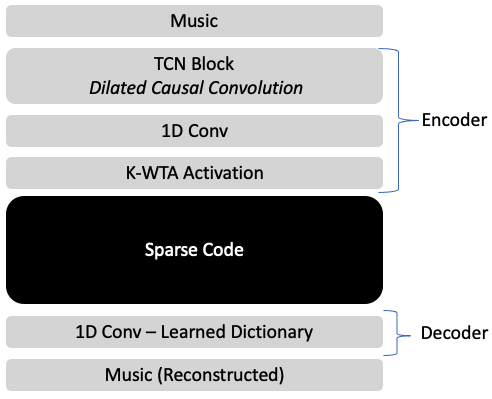
\includegraphics[width=\linewidth]{/Users/juanhuerta/personal_projects/code/shift_invariant_dictionary_learning/paper/images/tcn.png}
  \caption{Diagram depicting the Temporal CONV-WTA Autoencoder. The TCN Block can have arbitrary depth, and is not required to construct a dictionary but useful to extract features}
  \label{fig:bt1}
\end{figure}

\begin{figure*}[ht]
  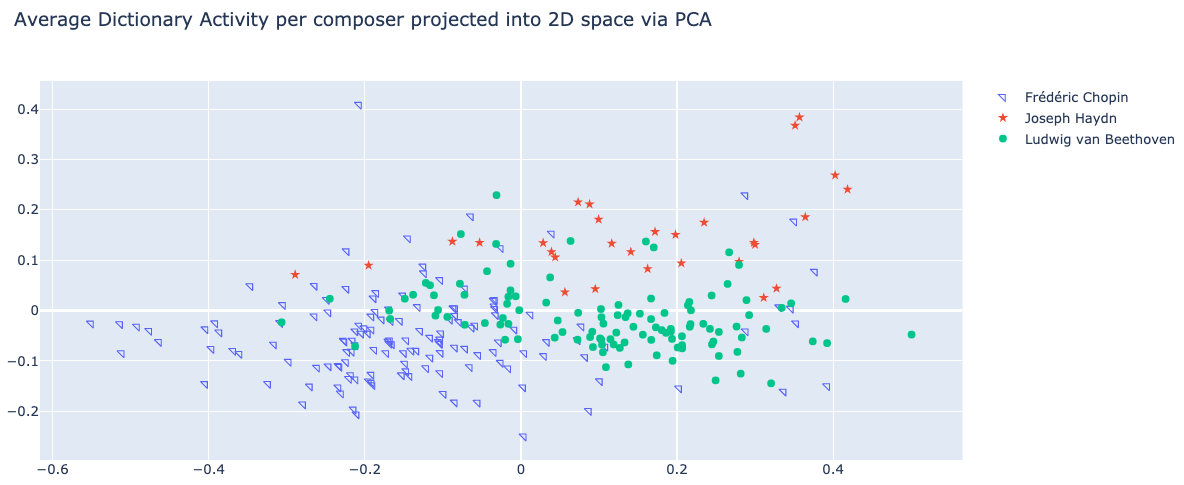
\includegraphics[width=\linewidth]{/Users/juanhuerta/personal_projects/code/shift_invariant_dictionary_learning/paper/images/newplot.png}
  \caption{After training the model on the MAESTRO dataset we can encode music of arbitrary length, average atom activity (rows of sparse code), and perform PCA for visualization }
    \label{fig:b4}
\end{figure*}




\section{Experiments}
\label{ssec:experiments}

We show a few applications of our CONV-WTA model, de-noising musical ideas, unsupervised learning of composer styles, and music generation. We do this for two distinct datasets with different MIDI encodings.


\subsection{Datasets}
\label{ssec:experiments}

Two distinct datasets are used: MAESTRO  \cite{hawthorne2018enabling}, and Groove \cite{groove2019} with two distinct MIDI representations (see Table 1 for more details).

\begin{table*}[ht]
    \centering
    \begin{tabular}{p{0.15\linewidth} | p{0.15\linewidth} | p{0.1\linewidth}  | p{0.45\linewidth} }
      Dataset  & Size  & Instrument &  MIDI Representation\\ \hline
      MAESTRO  & 1020 (Hrs)   & Piano &  One-hot encoding over 388 different MIDI events. Music has an arbitrary length \cite{DBLP:journals/corr/abs-1808-03715} \\
        \hline
        Groove & 3.6 (Hrs)  & Drum &  T timesteps (one per 16th note) and 27 MIDI events. We use fixed length 64 time step sections \cite{groove2019} \\
    \end{tabular}
    \caption{Details for the datasets used to train the Fully Convolutional Temporal Autoencoder (FCTA) }
    \label{tab:my_label}
\end{table*}

\subsection{Model Implementation}
Both models were implemented in Pytorch, with MSE loss on reconstruction, and AdamW optimizer. The model implementation differs slightly for the two datasets. 
 \\
\textbf{MAESTRO Model: } The architecture is illustrated in Figure 1. The TCN layer uses a [1,8,16,24] feature map, and a dictionary size of 1000 along with a decaying k-WTA\footnote{In the original paper k-WTA is applied after training the encoder. We use the k-WTA activation during training for lower GPU memory requirements, and the decaying k showed to achieve a higher accuracy}. The training begins with $k=100$ and decay to $k=75$ over $60$ epochs. The convolutions are non-overlapping strides, meaning every kernel-length time step is only made up of one column in our sparse code. This helps to reduce memory requirements and find repeating sections over a fixed kernel length. A batch size of 1 is used, this allows us to train on variable length music since our autoencoder is fully convolutional.  However our sparse representation can also be variable length. \\ 
\textbf{Groove Model: } The architecture is illustrated in Figure 1, however since the Groove drum representation is not very dense, we do not use a TCN layer. The  dictionary size is 100 along with a decaying k-WTA with $k=4$ and decay to $k=1$ over $1000$ epochs. The convolutions are  also non-overlapping strides. The full dataset is used with no batching. The dataset is processed to match 120 bpm, 4/4 time signature and only train on 1 bar of music. For this dataset we have a good understanding of repeating time intervals and structure, unlike the MAESTRO dataset.


\begin{figure*}[ht]
  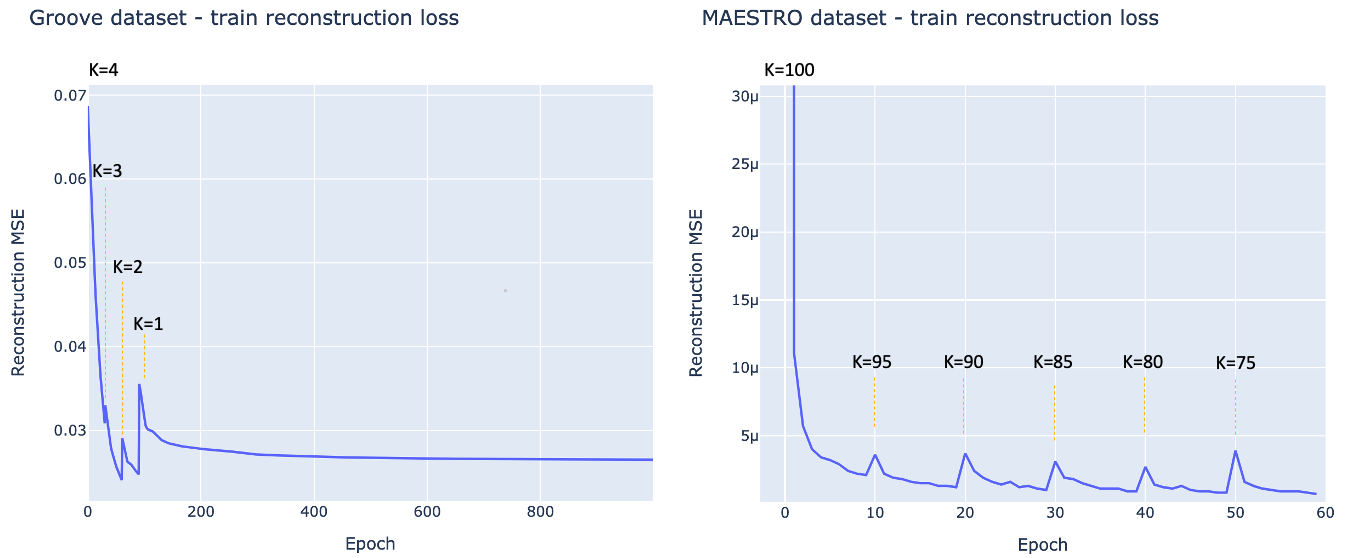
\includegraphics[width=\linewidth]{/Users/juanhuerta/personal_projects/code/shift_invariant_dictionary_learning/paper/images/maestro.png}
  \caption{ Reconstruction loss of the Temporal Convolutional Winner-Take-All (CONV-WTA) autoencode for MAESTRO and Groove training data. The value of k is decaying as we progress training$\textsuperscript{1}$ }
  \label{fig:boat2}
\end{figure*}


\subsection{Music Reconstruction}
\label{ssec:first}

 \textbf{De-noising Musical Ideas: } Dictionary learning has successfully been shown to de-noise images  \cite{Beckouche_2013}. By simply reconstructing our musical signal with a limited dictionary, our signal should dismiss “noisy” features that are not shift-invariant such as  inconstant musical ideas; moreso recognizing where music introduces shift-variant patterns can be useful for music analysis. 
 \\
 \textbf{Keep N Active Atoms: } The sparse coding’s ability to recognize the most used atoms in the dictionary enables a low dimensional feature extraction for machine learning tasks. We believe that this could be applied to music reduction wherein the complexity of the arrangement is reduced to a simpler transcription and parts in an unsupervised way.
 %And Music Segmentation (Discretization) wherein various musical ideas used in a piece of music are isolated from the piece itself. Such segmented ideas could be used in analysis or creatively repurposed to generate new music.

\subsection{Unsupervised Learning of Composer Styles }
We apply our model to a dataset that includes multiple composers to see if different composers utilize different shift-invariant patterns. After training, we encode music of arbitrary length, average atom activity (average rows of sparse code), and perform PCA for visualization. The result, as shown in Figure 2, illustrates separation and clustering of three distinct composer styles, and agrees with our assumption, for instance, that Haydn is stylistically closer to Beethoven than he is to Chopin. This sparse representation can also be used to measure similarity between composers by comparing distance of centroids between clusters, and we plan to utilize such measurement to aid music analysis and creation.

\subsection{Generating New Music}
 \textbf{Interpolating Sparse Code: } To generate new music, we encode existing music and interpolate between sparse codes\footnote{The interpolation result is better if the sections have similar musical ideas. We can use Cos similarity between the encodings to find similar musical sections to interpolate.}. For drum generation, all of the sections are fixed length whereas for the piano generation a variable length sparse code is used. To interpolate variable length code we can fix the input size, or interpolate specific time intervals of the sparse code.
 \\
 \textbf{Swapping Atoms: } Another method to generate new music is to measure the most active atoms in the dictionary from a musical section (row in the sparse code), and replace them with the most active atoms from a different musical section. This can be used as a tool for artists to freely re-mix and merge features and can offer a unique way to re-compose their own version of a given music.

%% NOTE: NLP4MusA desn't need DOI.
% BEGIN: remove
% \textbf{Digital Object Identifiers}:  As part of our work to make ACL
% materials more widely used and cited outside of our discipline, ACL
% has registered as a CrossRef member, as a registrant of Digital Object
% Identifiers (DOIs), the standard for registering permanent URNs for
% referencing scholarly materials.  As of 2017, we are requiring all
% camera-ready references to contain the appropriate DOIs (or as a
% second resort, the hyperlinked ACL Anthology Identifier) to all cited
% works.  Thus, please ensure that you use Bib\TeX\ records that contain
% DOI or URLs for any of the ACL materials that you reference.
% Appropriate records should be found for most materials in the current
% ACL Anthology at \url{http://aclanthology.info/}.
%
% As examples, we cite \cite{P16-1001} to show you how papers with a DOI
% will appear in the bibliography.  We cite \cite{C14-1001} to show how
% papers without a DOI but with an ACL Anthology Identifier will appear
% in the bibliography.  

%  As reviewing will be double-blind, the submitted version of the papers
%  should not include the authors' names and affiliations. Furthermore,
%  self-references that reveal the author's identity, \emph{e.g.},
%  \begin{quote}
%  ``We previously showed \cite{Gusfield:97} ...''  
%  \end{quote}
%  should be avoided. Instead, use citations such as 
%  \begin{quote}
%  ``\citeauthor{Gusfield:97} \shortcite{Gusfield:97}
%  previously showed ... ''
%  \end{quote}

% Any preliminary non-archival versions of submitted papers should be listed in the submission form but not in the review version of the paper. NLP4MusA reviewers are generally aware that authors may present preliminary versions of their work in other venues, but will not be provided the list of previous presentations from the submission form. 
% END: remove




%\section{Discussion}
%\label{ssec:discussion}
%
%There are multiple benefits to this sequence learning methodology. The first is such as simplicity and felxibilty, the TCN autoencocoder is a simple to implemnt arquitecture and requires any abitrary size combinations of multivariate musical signals.Also the size of the model for both Magenta and Groove are 877 KB and 750 KB respectively. In comparison, googles Performance RNN--LSTM-based recurrent neural network--is ~25MB, and other transformer based models can be GBs in size. 
%
%In addition, our method allows for incorporating known structural information into a model prior to trainng. and finally we have the most imporant benifit is the sparse representatoin and learned dictionaries, as we have shown this can be used for mutiple applications and analysis. 
%
%The performance on the recustruction and generation on for the drum Grove dataset  was significantly better than the piano (MAESTRO dataset). This is in part because the dataset was pre-proccessed to match with kernel size, and the drum sections were the same length and have lower dimensionality. 



% Min: no longer used as of ACL 2019, following ACL exec's decision to
% remove this extra workflow that was not executed much.
% BEGIN: remove
%% \section{XML conversion and supported \LaTeX\ packages}

%% Following ACL 2014 we will also we will attempt to automatically convert 
%% your \LaTeX\ source files to publish papers in machine-readable 
%% XML with semantic markup in the ACL Anthology, in addition to the 
%% traditional PDF format.  This will allow us to create, over the next 
%% few years, a growing corpus of scientific text for our own future research, 
%% and picks up on recent initiatives on converting ACL papers from earlier 
%% years to XML. 

%% We encourage you to submit a ZIP file of your \LaTeX\ sources along
%% with the camera-ready version of your paper. We will then convert them
%% to XML automatically, using the LaTeXML tool
%% (\url{http://dlmf.nist.gov/LaTeXML}). LaTeXML has \emph{bindings} for
%% a number of \LaTeX\ packages, including the ACL 2019 stylefile. These
%% bindings allow LaTeXML to render the commands from these packages
%% correctly in XML. For best results, we encourage you to use the
%% packages that are officially supported by LaTeXML, listed at
%% \url{http://dlmf.nist.gov/LaTeXML/manual/included.bindings}
% END: remove

\section{Conclusion}

%There are multiple benefits to this sequence learning methodology. The first is such as simplicity and felxibilty, the TCN autoencocoder is a simple to implemnt arquitecture and requires any abitrary size combinations of multivariate musical signals.Also the size of the model for both Magenta and Groove are 877 KB and 750 KB respectively. In comparison, googles Performance RNN--LSTM-based recurrent neural network--is ~25MB, and other transformer based models can be GBs in size. 
%
%In addition, our method allows for incorporating known structural information into a model prior to trainng. and finally we have the most imporant benifit is the sparse representatoin and learned dictionaries, as we have shown this can be used for mutiple applications and analysis. 
%


We have shown that a Temporal CONV-WTA Autoencoder can learn a sparse representation of arbitrary length symbolic musical signal. This shift-invariant, sparse representation can be used to analyze features, de-noise, extract style, and to generate musical content in a structured or unstructured way. The reconstruction and generation for the drum (Groove) dataset was significantly better than the piano (MAESTRO) dataset. This is in part because the drum dataset was preprocessed to match with the kernel size, all drum sections were the same length, and had lower dimensionality in comparison. \\
In the future, we hope to use a larger and more diverse dataset, improve reconstruction performance, and apply similar preprocessing to the piano data as done for the drum data. We also plan to further develop applications of this technology and build tools for artists.
\\
\\
\\
\\
\\
%\section*{Acknowledgments}
%
%The acknowledgments should go immediately before the references.  Do
%not number the acknowledgments section. Do not include this section
%when submitting your paper for review. \\

%\noindent \textbf{Preparing References:} \\
%Include your own bib file like this:
%\verb|\bibliographystyle{nlp4MusA_natbib}|
%\verb|\bibliography{nlp4MusA}| 
%
%where \verb|nlp4MusA| corresponds to a nlp4MusA.bib file.
\bibliography{nlp4MusA}
\bibliographystyle{nlp4MusA_natbib}


%\appendix
%
%\section{Appendices}
%\label{sec:appendix}
%Appendices are material that can be read, and include lemmas, formulas, proofs, and tables that are not critical to the reading and understanding of the paper. 
%Appendices should be \textbf{uploaded as supplementary material} when submitting the paper for review. Upon acceptance, the appendices come after the references, as shown here. Use
%\verb|\appendix| before any appendix section to switch the section
%numbering over to letters.
%
%
%\section{Supplemental Material}
%\label{sec:supplemental}
%Submissions may include non-readable supplementary material used in the work and described in the paper. Any accompanying software and/or data should include licenses and documentation of research review as appropriate. Supplementary material may report preprocessing decisions, model parameters, and other details necessary for the replication of the experiments reported in the paper. Seemingly small preprocessing decisions can sometimes make a large difference in performance, so it is crucial to record such decisions to precisely characterize state-of-the-art methods. 
%

\end{document}
